\documentclass[11pt]{article}

\usepackage[a4paper,margin=1in]{geometry}
\usepackage{booktabs}
\usepackage{array}
\usepackage{longtable}
\usepackage{tabularx}
\usepackage{enumitem}
\usepackage{xcolor}
\usepackage{hyperref}
\usepackage{tikz}
\usetikzlibrary{arrows.meta,positioning,shapes.geometric}

\hypersetup{
  colorlinks=true,
  linkcolor=blue!60!black,
  urlcolor=blue!60!black,
  citecolor=blue!60!black
}

\newcommand{\checkpoint}{\texttt{threads\_pilot\_v1\_0081}}
\newcommand{\dataset}{\texttt{manual\_records\_checkpoint\_0081.jsonl}}
\newcommand{\repoartifact}[1]{\texttt{\detokenize{#1}}}

\title{Threads Scam-Content Research Checkpoint 0081\\
\large CIB-Approved Technical Report for Evidence-System Review}
\author{Meta Threads Scam-Content Research 2026}
\date{2026-04-27}

\begin{document}
\maketitle

\begin{abstract}
This technical report summarizes the CIB-approved 78-record research checkpoint for a governed Threads scam-content evidence system.
The checkpoint is designed for research review, rule-family learning, annotation calibration, and governance auditability.
It is not a production detector, legal fraud determination, or prevalence estimate.
The checkpoint contains 36 scam-labeled records, 24 non-scam records, 13 uncertain records, and 5 insufficient-evidence records.
Strict validation passed with 0 errors and 0 warnings.
A transparent rule-baseline smoke evaluation over 60 binary-evaluable records achieved precision 0.829, recall 0.944, and F1 0.883, with 7 false positives and 2 false negatives.
The results support continued human review, targeted confirmed-pointer intake when new evidence is explicitly authorized, and strong caution against unbounded crawler/browser expansion or model training from this checkpoint alone.
\end{abstract}

\section*{Executive Summary}

Checkpoint \checkpoint{} is a CIB-approved research checkpoint consisting of 78 strict-valid, redacted records.
It is intended to make the evidence system reviewable: reviewers should be able to inspect how items were collected, redacted, annotated, second-reviewed, validated, and summarized without exposing raw Threads evidence in tracked artifacts.

The checkpoint's main contribution is not volume.
Its main contribution is sharper distinction among four categories:

\begin{enumerate}[leftmargin=*]
  \item confirmed scam-like investment or private-channel funnels;
  \item anti-scam warning hard negatives;
  \item high-risk trust-building starters that require more context;
  \item thin fragments that must remain \texttt{uncertain} or \texttt{insufficient\_evidence}.
\end{enumerate}

The recommended next action is reviewer-facing package delivery and report refinement.
This checkpoint does not authorize item \texttt{0082}, broad crawler/browser expansion, embedding or model training, production detection, or legal fraud determinations.

\section{Scope and Governance Boundary}

This report covers the CIB-approved checkpoint \checkpoint{} and the repo-safe artifacts that support it.
The dataset file is \dataset{}, stored as a local/interim research artifact.
Tracked reports contain only redacted, normalized, hashed, counted, or presence-only evidence representations.

\begin{table}[h]
\centering
\caption{Checkpoint identity and governance status.}
\begin{tabularx}{\textwidth}{@{}lX@{}}
\toprule
Field & Value \\
\midrule
Checkpoint & \checkpoint{} \\
Records & 78 strict-valid records \\
Approval & CIB-approved research checkpoint \\
Dataset file & \dataset{} \\
Primary synthesis & \repoartifact{experiments/evaluation-notes/0089-checkpoint-0081-cib-approved-synthesis.md} \\
Decision record & \repoartifact{decision-log/0105-approve-cib-78-record-checkpoint-synthesis.md} \\
Package index & \repoartifact{reports/checkpoint-0081-approved-package-index.md} \\
Use & Redacted evidence-system checkpoint review \\
\bottomrule
\end{tabularx}
\end{table}

\subsection{Explicit Non-Claims}

This checkpoint does not claim:

\begin{itemize}[leftmargin=*]
  \item platform prevalence of scam content on Threads;
  \item legal fraud determination for any person or entity;
  \item production detector readiness;
  \item permission to start item \texttt{0082};
  \item permission for broad browser-session or crawler expansion;
  \item permission for embedding/model training.
\end{itemize}

\section{Evidence Pipeline}

The evidence pipeline separates raw controlled evidence from tracked research artifacts.
Raw source material, if captured, remains in controlled storage.
The tracked repo receives only redacted records, aggregate metrics, rule-family summaries, decision logs, and validation provenance.

\begin{figure}[h]
\centering
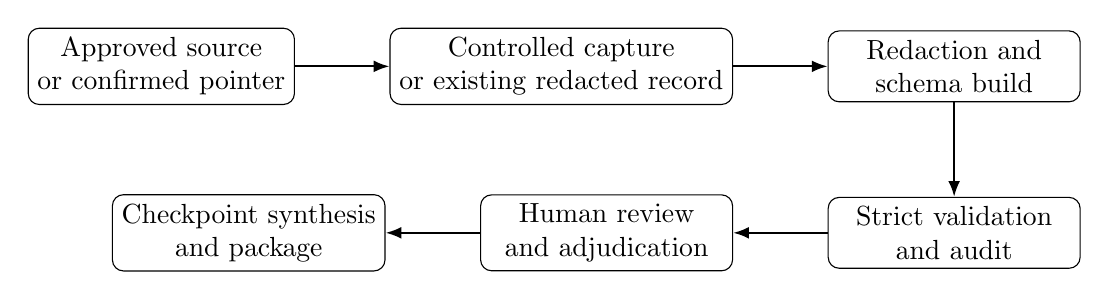
\begin{tikzpicture}[
  node distance=1.2cm,
  box/.style={draw, rounded corners, align=center, minimum width=3.2cm, minimum height=0.9cm},
  arrow/.style={-{Latex[length=2mm]}, thick}
]
\node[box] (pointer) {Approved source\\or confirmed pointer};
\node[box, right=of pointer] (capture) {Controlled capture\\or existing redacted record};
\node[box, right=of capture] (redact) {Redaction and\\schema build};
\node[box, below=of redact] (validate) {Strict validation\\and audit};
\node[box, left=of validate] (review) {Human review\\and adjudication};
\node[box, left=of review] (synthesis) {Checkpoint synthesis\\and package};
\draw[arrow] (pointer) -- (capture);
\draw[arrow] (capture) -- (redact);
\draw[arrow] (redact) -- (validate);
\draw[arrow] (validate) -- (review);
\draw[arrow] (review) -- (synthesis);
\end{tikzpicture}
\caption{Repo-safe evidence pipeline. Raw evidence does not enter tracked reports.}
\end{figure}

\section{Dataset Composition}

\subsection{Labels and Risk}

The checkpoint has 78 records.
The label and risk distributions are shown in Table~\ref{tab:label-risk}.

\begin{table}[h]
\centering
\caption{Label and risk distribution at checkpoint 0081.}
\label{tab:label-risk}
\begin{tabular}{@{}lrr@{}}
\toprule
Category & Count & Share \\
\midrule
\texttt{scam} & 36 & 46.2\% \\
\texttt{non\_scam} & 24 & 30.8\% \\
\texttt{uncertain} & 13 & 16.7\% \\
\texttt{insufficient\_evidence} & 5 & 6.4\% \\
\midrule
\texttt{high} risk & 36 & 46.2\% \\
\texttt{medium} risk & 11 & 14.1\% \\
\texttt{low} risk & 31 & 39.7\% \\
\bottomrule
\end{tabular}
\end{table}

\subsection{Evidence Sufficiency, Source Mix, and Content Shape}

Evidence sufficiency remains uneven, which is expected for an early governed checkpoint.
Partial and insufficient cases are retained because forcing a label would reduce scientific reliability.

\begin{table}[h]
\centering
\caption{Evidence sufficiency and source mix.}
\begin{tabular}{@{}lrr@{}}
\toprule
Measure & Count & Share \\
\midrule
\texttt{sufficient} evidence & 22 & 28.2\% \\
\texttt{partial} evidence & 45 & 57.7\% \\
\texttt{insufficient} evidence & 11 & 14.1\% \\
\midrule
\texttt{manual\_public} source & 60 & 76.9\% \\
\texttt{stakeholder\_provided} source & 18 & 23.1\% \\
\bottomrule
\end{tabular}
\end{table}

\begin{table}[h]
\centering
\caption{Content shape distribution.}
\begin{tabular}{@{}lr@{}}
\toprule
Content shape & Count \\
\midrule
\texttt{link\_or\_redirect} & 37 \\
\texttt{text\_only} & 20 \\
\texttt{reply\_context} & 16 \\
\texttt{text\_image\_post} & 4 \\
\texttt{screenshot\_ocr} & 1 \\
\bottomrule
\end{tabular}
\end{table}

\section{Checkpoint Evolution}

Checkpoint 0081 builds on checkpoint 0055, local item 0076, second-review adjudication, and two completed confirmed-pointer records.
Figure~\ref{fig:evolution} summarizes the evolution.

\begin{figure}[h]
\centering
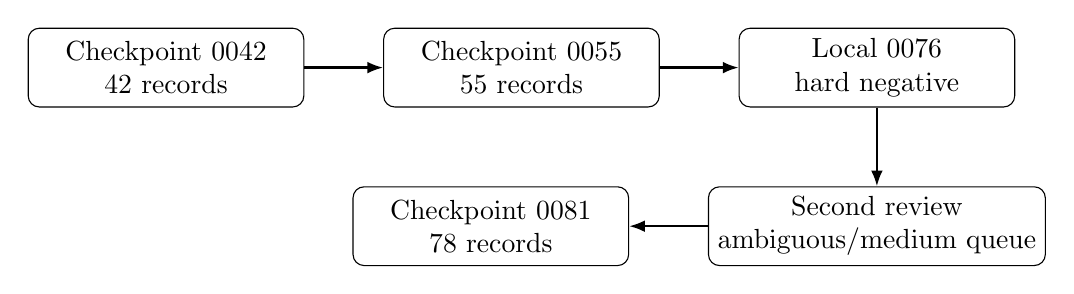
\begin{tikzpicture}[
  node distance=1.0cm,
  stage/.style={draw, rounded corners, align=center, minimum width=3.5cm, minimum height=1.0cm},
  arrow/.style={-{Latex[length=2mm]}, thick}
]
\node[stage] (c42) {Checkpoint 0042\\42 records};
\node[stage, right=of c42] (c55) {Checkpoint 0055\\55 records};
\node[stage, right=of c55] (c76) {Local 0076\\hard negative};
\node[stage, below=of c76] (second) {Second review\\ambiguous/medium queue};
\node[stage, left=of second] (c81) {Checkpoint 0081\\78 records};
\draw[arrow] (c42) -- (c55);
\draw[arrow] (c55) -- (c76);
\draw[arrow] (c76) -- (second);
\draw[arrow] (second) -- (c81);
\end{tikzpicture}
\caption{Checkpoint evolution from initial evidence-system review to the CIB-approved 78-record checkpoint.}
\label{fig:evolution}
\end{figure}

\begin{table}[h]
\centering
\caption{Delta from checkpoint 0055 to checkpoint 0081.}
\begin{tabular}{@{}lrrr@{}}
\toprule
Metric & Checkpoint 0055 & Checkpoint 0081 & Delta \\
\midrule
Total records & 55 & 78 & +23 \\
\texttt{scam} & 17 & 36 & +19 \\
\texttt{non\_scam} & 23 & 24 & +1 \\
\texttt{uncertain} & 9 & 13 & +4 \\
\texttt{insufficient\_evidence} & 6 & 5 & -1 \\
\texttt{high} risk & 17 & 36 & +19 \\
\texttt{medium} risk & 7 & 11 & +4 \\
\texttt{low} risk & 31 & 31 & 0 \\
\bottomrule
\end{tabular}
\end{table}

\section{Annotation and Second Review}

Decision \repoartifact{0101} authorized a bounded second review of existing redacted records with \texttt{uncertain}, \texttt{insufficient\_evidence}, or \texttt{medium} risk status.
No new evidence collection was authorized by that review.

\begin{table}[h]
\centering
\caption{Second-review outcome categories.}
\begin{tabularx}{\textwidth}{@{}lX@{}}
\toprule
Outcome & Item IDs \\
\midrule
Promoted to \texttt{scam}/\texttt{high} &
\texttt{0012}, \texttt{0017}, \texttt{0020}, \texttt{0021}, \texttt{0025}, \texttt{0049}, \texttt{0050}, \texttt{0051}, \texttt{0052}, \texttt{0055}, \texttt{0056}, \texttt{0058}, \texttt{0062}, \texttt{0067}, \texttt{0068}, \texttt{0071}, \texttt{0075} \\
Kept \texttt{uncertain}/\texttt{medium} &
\texttt{0027}, \texttt{0047}, \texttt{0057}, \texttt{0064}, \texttt{0065}, \texttt{0066}, \texttt{0069}, \texttt{0070}, \texttt{0072} \\
Kept \texttt{uncertain}/\texttt{low} &
\texttt{0059}, \texttt{0060}, \texttt{0061}, \texttt{0063} \\
Kept or moved to \texttt{insufficient\_evidence}/\texttt{medium} &
\texttt{0073}, \texttt{0074} \\
Kept \texttt{insufficient\_evidence}/\texttt{low} &
\texttt{0048}, \texttt{0053}, \texttt{0054} \\
\bottomrule
\end{tabularx}
\end{table}

\section{Rule-Family Findings}

The checkpoint supports rule-family learning from feature combinations, not isolated keywords.
Table~\ref{tab:rules} summarizes the main rule families and protected boundaries.

\begin{longtable}{@{}p{0.28\textwidth}p{0.38\textwidth}p{0.24\textwidth}@{}}
\caption{Rule-family findings and protected boundaries.}
\label{tab:rules}\\
\toprule
Rule family & Stronger when combined with & Boundary \\
\midrule
\endfirsthead
\toprule
Rule family & Stronger when combined with & Boundary \\
\midrule
\endhead
Profit proof and testimonial evidence &
External-link, private-channel, stock-tip, or group-conversion context &
Past performance alone is not enough. \\
Private-channel migration &
Investment, crypto, day-trading, loss-rescue, contact cue, or reply-level funnel &
Messaging-app mention alone is not enough. \\
Comment-account reinforcement &
Profit claims, testimonial claims, or coordinated reassurance &
Ordinary comments are not enough. \\
Public stock-tip or named-stock reassurance &
Conversion context, group/contact link, reassurance, guarantee, or follow action &
Ordinary market discussion is not enough. \\
Profit-plus-social-good framing &
Presumed future profit plus external-link, guarantee, or unrealistic-benefit signal &
Ordinary charity language is not enough. \\
Reply contact hijack or anti-scam camouflage &
``Safe'' contact path, group entry, daily watchlist, or holdings-viewpoint cue &
Anti-scam words do not neutralize a funnel. \\
Anti-scam warning hard negative &
Victim-prevention orientation without the author's own conversion path &
Scam-method vocabulary alone is not scam. \\
Market-scope or trading-psychology starter &
Private-message, community, stock-tip, reassurance, guarantee, or contact cue &
Single-sentence fragments remain weak. \\
\bottomrule
\end{longtable}

\section{Baseline Smoke Evaluation}

The rule baseline is a transparent triage baseline.
It is useful for finding review candidates and stress-testing the rule library.
It is not a production model.

\begin{table}[h]
\centering
\caption{Rule-baseline smoke metrics.}
\begin{tabular}{@{}lr@{}}
\toprule
Metric & Value \\
\midrule
Binary metric items & 60 \\
Accuracy & 0.850 \\
Precision & 0.829 \\
Recall & 0.944 \\
F1 & 0.883 \\
True positives & 34 \\
True negatives & 17 \\
False positives & 7 \\
False negatives & 2 \\
Triage exact agreement & 0.590 \\
\bottomrule
\end{tabular}
\end{table}

The two false negatives are important.
They show that the current rule baseline can still miss scam/high cases after human adjudication.
Therefore, this checkpoint supports continued human review and rule refinement rather than automation-only deployment.

\section{Limitations}

\begin{enumerate}[leftmargin=*]
  \item The checkpoint is source-skewed: 60 of 78 records are \texttt{manual\_public}.
  \item The checkpoint is collection-method-skewed: 60 of 78 records use \texttt{manual\_capture}.
  \item Many records have empty or partial reply context.
  \item OCR is under-tested, with only one \texttt{screenshot\_ocr} content-shape record.
  \item Link, contact, and identity evidence is redacted or represented at category level in tracked artifacts.
  \item Duplicate and near-duplicate traces remain important for interpretation.
  \item Confirmed pointers are high-yield for rule learning but cannot support prevalence estimates.
\end{enumerate}

\section{Reviewer Decision Points}

Reviewers should decide whether the package is ready for checkpoint delivery, and whether any report edits are required before broader sharing.

\begin{table}[h]
\centering
\caption{Reviewer response table.}
\begin{tabularx}{\textwidth}{@{}lX@{}}
\toprule
Field & Response \\
\midrule
Checkpoint reviewed & \checkpoint{} \\
Delivery status & \texttt{approve\_for\_checkpoint\_delivery} / \texttt{approve\_with\_minor\_edits} / \texttt{revise\_before\_delivery} / \texttt{block\_delivery} \\
Required edits & \\
Additional reviewer roles & legal/privacy / domain / technical / stakeholder \\
New evidence collection authorized? & \texttt{no}, unless a separate capped decision is recorded \\
Notes & \\
\bottomrule
\end{tabularx}
\end{table}

\section{Conclusion}

Checkpoint 0081 is suitable as the current CIB-approved research checkpoint for evidence-system review.
It strengthens the rule library, clarifies hard-negative boundaries, and shows that second review can reduce false-negative risk without opening new collection.
At the same time, the checkpoint remains too small and source-skewed for prevalence claims, production deployment, or model training.
The next appropriate step is reviewer-facing package delivery and report refinement.

\appendix

\section{Repo-Safe Artifact Map}

\begin{longtable}{@{}p{0.38\textwidth}p{0.52\textwidth}@{}}
\toprule
Artifact & Purpose \\
\midrule
\endfirsthead
\toprule
Artifact & Purpose \\
\midrule
\endhead
\repoartifact{reports/checkpoint-0081-approved-package-index.md} & Canonical package index. \\
\repoartifact{reports/checkpoint-0081-executive-addendum.md} & Short reviewer entry point. \\
\repoartifact{experiments/evaluation-notes/0089-checkpoint-0081-cib-approved-synthesis.md} & Detailed checkpoint synthesis. \\
\repoartifact{experiments/evaluation-notes/0088-existing-ambiguous-medium-second-review-synthesis.md} & Second-review synthesis. \\
\repoartifact{decision-log/0105-approve-cib-78-record-checkpoint-synthesis.md} & CIB approval decision. \\
\repoartifact{governance/pilot-launch/run_index.md} & Run and checkpoint index. \\
\repoartifact{docs/06-annotation-guideline-v1.md} & Annotation guideline and boundaries. \\
\repoartifact{data-contracts/thread_item_schema_v1.json} & Thread item schema. \\
\repoartifact{data-contracts/labeling_schema_v1.json} & Labeling schema. \\
\bottomrule
\end{longtable}

\section{Raw Evidence Boundary}

This report intentionally excludes raw Threads URLs, handles, screenshots, raw post text, raw reply text, contact IDs, stock names, stock codes, price values, credentials, browser/session artifacts, exact controlled-store paths, and stakeholder case IDs.
Those exclusions are research controls, not omissions of the evidence process.

\end{document}
